\documentclass[]{llncs} 
\usepackage{verbatim}
\usepackage{tikz}
\usetikzlibrary{arrows,shapes}
\usepackage{graphics}
\usepackage{url}
\usepackage{amsmath}

\author{Marijn Heule \and Valentin Mayer-Eichberger}

\institute{Department of Software Technology\\
Delft University of Technology\\
\email{marijn@heule.nl} \\
\email{mayereichberger@gmail.com}
}

\title{Encoding the Spinpossible Puzzle in SAT}

\newcommand{\code}[1]{\verb|#1|} 
\newcommand{\spintable}[9]{ 
\node [matrix,ampersand replacement=\&,nodes={minimum size=6mm}]
%,nodes={fill=blue!20,minimum size=5mm}] 
    {
        \node (n11) {#1}; \& \node (n12) {#2}; \& \node {#3}; \\ 
        \node {#4}; \& \node{#5}; \& \node {#6}; \\ 
        \node {#7}; \& \node{#8}; \& \node (n33) {#9}; \\ 
    }; 
\draw[gray] (n11.north west) rectangle (n33.south east);
}

\newcommand{\TODO}[1]{ {\color{red}{TODO: #1} }}
\newcommand{\com}[1]{ {\color{blue}{--- #1 ---}}}

\begin{document} 

\maketitle

\section{Introduction}

\subsection{Spinpossible}

\emph{Spinpossible}\footnote{See \url{www.spinpossible.com} for further information.} is a new combinatorial game in the
line of Rubiks cube or Sudoku. Given a $3\cdot 3$ matrix of numbers 1 to 9 the task is to rearrange the numbers with
rectangular 180 degree rotations such that they are at their natural position. The rotation is a pointwise rotation
through the center of the rectangle. The solved matrix is as follows.

\begin{center}
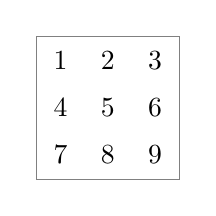
\begin{tikzpicture}
\spintable{1}{2}{3}{4}{5}{6}{7}{8}{9}
\end{tikzpicture}
\end{center}

An additional difficulty is the orientation of the numbers. Through a rotation (also called spin) the numbers change
orientation and can also appear up side down. Numbers up side down are denoted here as negated numbers, so all numbers
within the rectangle change sign after the rotation.  

The following example demonstrates a stepwise solution by rectangular rotations. In the given problem all but numbers 1
and 9 are at their correct position, so the task is to swap 1 and 9 back. The spins are marked by a red
rectangle.

\vspace{0.5cm}

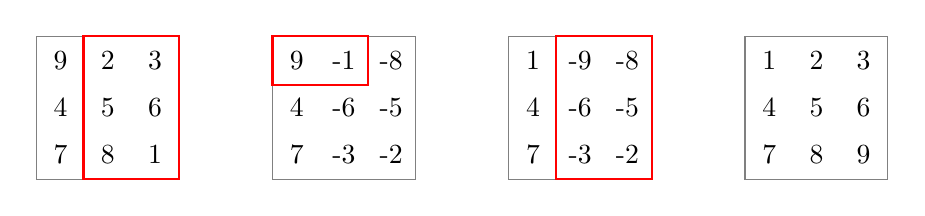
\begin{tikzpicture} 
\spintable{9}{2}{3}{4}{5}{6}{7}{8}{1}
\draw[red,thick] (n12.north west) rectangle (n33.south east);
\begin{scope}[xshift=3cm] 
\spintable{9}{-1}{-8}{4}{-6}{-5}{7}{-3}{-2}
\draw[red, thick] (n11.north west) rectangle (n12.south east);
\end{scope}
\begin{scope}[xshift=6cm] 
\spintable{1}{-9}{-8}{4}{-6}{-5}{7}{-3}{-2}
\draw[red, thick] (n12.north west) rectangle (n33.south east);
\end{scope}
\begin{scope}[xshift=9cm] 
\spintable{1}{2}{3}{4}{5}{6}{7}{8}{9}
\end{scope}
\end{tikzpicture} 

\vspace{0.5cm}

Note that this is a minimal solution in the sense that there is no solution with less spins. However, it is not the
only solution with three spins. 

The game can be interpreted as a planning problem considering the matrix as states, the solved board as the final state and
the spins as actions. The task is then to find a plan - a sequence of actions - to reach the final state.

Interesting questions arise in analyzing the spinpossible game. What is the minimal number of spins to solve all initial
boards? Which computational approach can solve boards in reasonable time? The paper \cite{Sutherland2011} written by the
inventors of the game raises further mathematical questions. Our analysis in this paper  is computational and we will
explain how to solve spinpossible boards practically. \TODO{Give more questions and restructure, describe the
motivation} 

\subsection{Satisfiability Problem}

The basic idea is to translate the rules of the game and the initial board into a logical expression in conjunctive
normal form (CNF) that is then solved by a general purpose SAT solver. The model of such a formula contains the solution
to the given problem. The approach is thus not to create a special purpose algorithm to solve boards, but rather to use
a suitible representation language for such problems and apply programs that solve expressions in these language.
Regarding SAT solvers and CNF this approach has been successfully applied in several fields, as hardware and software
verification and synthesis, planning and scheduling problems \cite{Biere2009}. 

\TODO{Is Spinpossible $n\cdot m$ with a given number of steps $N$ really NP complete? How to transform 3SAT into
spinpossible? Alternatives...}


\section{SAT and Propositional Modeling}

Here we will give some the usual pointers to literature about encodings. (Rubiks cube, Garden of Eden, etc. ),
\cite{Chen2011}

The art of finding good encodings! How to learn the tricks! We would like to establish more knowledge about the what is
so far called  tricks.  We will show alternative encodings of spinpossible, present a reasonable benchmark and compare
encodings along with it.

\section{Encoding in SAT}

The basic CNF encoding uses three types of variables: State variables $x$, equality variables $e$ and transition
variables $t$. To describe the structure of the clauses we introduce the following index sets:

\begin{itemize}
\item $A := \{1,\dots,9\}$ the set of positions numbered in their natural order
\item $M := \{1,\dots,36\}$ the set of moves (arbitrary order)
\item $S_m$ the subset of $A$ corresponding to the squares touched by move $m \in M$
\item $d_m$ the distance of move $m \in M$ computes as the max + min element in $S_m$
\item $N$ refers to the number of moves.

\end{itemize}

\paragraph{State variables} The SAT encoding described in this paper . The meaning for variable $x_{i,j,k}$ is as
follows: if $x_{i,j,k}$ is assigned to true, then position $i$ contains symbol $j$ at time $k$.  There are a special state
variables $x_{i,0,k}$ to indicate whether the symbol on position $i$ is rotated. If $x_{i,0,k} = 1$ the symbol on position
$i$ at time $k$ is upside down.  

\paragraph{Fixing initial and final state} Using the following unit clauses, the state variables of the final state can
be fixed:

\begin{equation}
\bigwedge_{i=1}^9  (x_{i,i,N+1}) \land \bigwedge_{i=1}^9 \bigwedge_{j=0}^{i-1} (\bar x_{i,j ,N+1}) \land
\bigwedge_{i=1}^9 \bigwedge_{j=i+1}^{9} (\bar x_{i,j ,N+1})
\end{equation}

\paragraph{Equality constraints} The first type of auxiliary variables are {\em equality variables} $e_{i,k}$. The
meaning of these variables is as follows: if $e_{i,k}$ is assigned to true, then tile $i$ is not modified during move
$k$, or expressed in state variables: $\bar x_{i,j,k} \leftrightarrow \bar x_{i,j,k+1}$. The following clauses show the
{\em equality constraints} that define the equality variables:

\begin{equation}
\bigwedge_{i=1}^9 \bigwedge_{j=0}^9 \bigwedge_{k=0}^{N} \big( (\bar e_{i,k} \lor \bar x_{i,j,k} \lor x_{i,j,k+1}) \land
(\bar e_{i,k} \lor x_{i,j,k} \lor \bar x_{i,j,k+1}) \big )
\end{equation}

\paragraph{Transition constraints} The second type of auxiliary variables are {\em transition variables} $t_{k,m}$.
The meaning of these variables is as follows: if $t_{k,m}$ is assigned to true, then at time $k$ move $m$ is applied.
First we need clauses to ensure that at each step exactly one move is applied. For each more we need one clause of
length $|M|$ that enforces that at least one move is done. The equality variables are reused to make sure that for each $k$
at-most-one of the variables $t_{k,m}$ with $m \in M$ can be true. The clauses below describe the implementation.
Notice that this implementation also realizes that tiles that are not affected during move $m$ (i.e.\ $i \in A \setminus S_m$)
are made equal using the equality constraints.

\begin{equation}
\bigwedge_{k=0}^{N} (\bigvee_{m \in M} t_{k,m}) \land \bigwedge_{k=0}^{N} \bigwedge_{m \in M} \bigwedge_{i \in A
\setminus S_m} (\bar t_{k,m} \lor e_{i,k}) \land \bigwedge_{k=0}^{N} \bigwedge_{m \in M} \bigwedge_{i \in S_m} (\bar
t_{k,m} \lor \bar e_{i,k})
\end{equation}

Second, tiles have to change places. This is encoded as follows:

\begin{equation}
\bigwedge_{k=0}^{N} \bigwedge_{m \in M} \bigwedge_{i \in S_m} \bigwedge_{j=1}^9 \big( (\bar t_{k,m} \lor \bar x_{i,j,k}
\lor x_{d_m - i,j,k + 1} ) \land (\bar t_{k,m} \lor x_{i,j,k} \lor \bar x_{d_m - i,j,k + 1} ) \big)
\end{equation}

Third, the tiles that have changed places have to be rotated. This is done using the following clauses.

\begin{equation}
\bigwedge_{k=0}^{N} \bigwedge_{m \in M} \bigwedge_{i \in S_m} \big( (\bar t_{k,m} \lor x_{i,0,k} \lor x_{d_m - i,0,k +
1} ) \land (\bar t_{k,m} \lor \bar x_{i,0,k} \lor \bar x_{d_m - i,0,k + 1} ) \big)
\end{equation}


\subsection{Symmetry breaking predicates}

Spinpossible has many solution symmetries. First, we illustrate this by an example. We will denote by $I$ the initial
state and by $G$ the goal state. Let list $L$ refer to a solution being a sequence of moves that transform $I$ into $G$.
Consider a solution $L$ with the first move only spinning the tile with symbol $1$. We can construct $|L|$ symmetric
solutions as follows: remove the first move from $L$ and insert a move at position $i \in \{1,\ldots, |L|\}$ that only
flips the tile containing symbol $1$ in the state after $i-1$ moves.

A SAT solver is not aware of that a list of moves $L$ is symmetric with a list $L'$. As a consequence, it may explore
all symmetric sequences of moves during the search. It is common practice to deal with the problem by adding {\em
symmetry breaking predicates} (SBPs).

SBPs enforce an order to those moves that have no fixed position in a solution. There are three types of these kind of
moves. First, all moves that flip a single tile. Second, two moves $n$ and $m$ do not influence each other ($S_n \cap
S_m = \emptyset$).  Third,  one move $n$  is fully part of move $m$ ($S_n \subseteq S_m$).


\begin{equation}
B_m = \{ n \in M \mid n \leq m \mathrm{~and~} ( S_n \subseteq S_m \mathrm{~or~} S_n \supset S_m \mathrm{~or~} S_n \cap
S_m = \emptyset) \}
\end{equation}

The above definition of $B_m$ can be simplified in case the moves are sorted such that for all pairs of moves $n$, $m$
hold that if $n < m$, then $|S_n| \leq |S_m|$.

Given such a sorting, the check $S_n \supset S_m$ becomes redundant.

After computing for $m \in M$ each $B_m$, it is easy to generate the SBPs:

\begin{equation}
\bigwedge_{k=0}^{N} \bigwedge_{m \in M} \bigwedge_{n \in B_m} (\bar t_{k,m} \lor \bar t_{k+1,n}) 
\end{equation}

\TODO{Add further ideas of symmetry breaking}


\section{An Alternative Encoding}

Notice that this encoding works the way it is explained only for the $3\times 3$ spinpossible. Most of the ideas can,
however, be extended to larger size. The ideas behind the encoding are 1) consider dimensions separately in both state
variables and move variables 2) the move variables just identify one column/row and clauses restrict them to form a
rectangle and 3) equality variables are implicitly represented by replacing equality with the orientation variable in
two consecutive time steps. This last idea relies on the equality that a number is within the rectangle if and only if
it changes orientation at that time point. 

This encoding significantly reduces the number of variables, at the same time doubles the number of clauses and
increasing the length of clauses. In practice this encoding  preforms well on all benchmarks.

With help of the following sets we will introduce the variables and clauses:

\begin{itemize}
\item $V := \{1,\dots,9\}$ the set of numbers
\item $D := \{\downarrow,\rightarrow\} $ the set of dimensions
\item $C := \{0,1,2\}$ the set of possible positions per dimension
\item $I := \{1\ldots N\}$ the set  of moves, starting with move 1. Time point $N+1$ describes the final state. 
\end{itemize}

The following variables are all variables needed:

\begin{itemize} 

\item State variable $s_{d,i,v,c}$ where $d\in D, i \in I\cup \{N+1\}, v \in V$ and $c \in C$. The variable  is true if in  step $i$
number $v$ is in row or column $c$ (depending on $d$). 

\item Move variable $m_{d,i,c}$ ($d,c$ as above, $i\in I$). The variable is true if in step $i$ the row/column $c$ is
part of the rectangle. $d$ determines whether it is a row or a column. The set of all true move variables in step $i$
identifies the rotating rectangle in that step. 

\item Parity variable $p_{i,v}$ is true if in step $i$ number $v$ is up side down. 

\end{itemize}


\paragraph{Restriction on the rectangle.} 
%
%:-  c(C2), 
%    C1 < C2, C2 < C3,
%    move(D,K,C1), 
%    move(D,K,C3), 
%    not move(D,K,C2).

The move variables together form the rectangle. In order to restrict the
combination rectangles we need to enforce the following two things.

The following clauses express that at least one move variable is true in each dimension and there are no inconsistent rectangles  

\begin{equation}
\bigwedge_{d \in D}\bigwedge_{i\in I} \bigvee_{c\in C}  (m_{d,i,c}) \wedge \bigwedge_{d \in D} \bigwedge_{i \in I} (\bar
m_{d,i,1} \vee m_{d,i,2} \vee \bar m_{d,i,3})
\end{equation}

\paragraph{Restriction on state variables.} 
%
%:-  state(D,K,V,C1), state(D,K,V,C2), C1 != C2. 

A number can only occur once in each column/row

\begin{equation}
\bigwedge_{d \in D}\bigwedge_{i\in I} \bigwedge_{v\in V} \bigwedge_{c_1 \neq c_2} (\bar s_{d,i,v,c_1} \vee \bar
s_{d,i,v,c_2})
\end{equation}

and in each row, column there are exactly three numbers (requires cardinality encoding). \TODO{Write cardinality
restriction for state variables.} These clauses are in fact redundant. 

\paragraph{Initial and final state.}
%
%:-  final(N), v(V), not state(x,N,V,((V-1) #div n)+1).
%:-  final(N), v(V), not state(y,N,V,((V-1) #mod n)+1).
%:-  final(N), parity(N,V).

The initial state is inferred from the problem configuration by setting for each number the corresponding state variable
to true. I.e. if number $6$ is at position $2,3$ then variable $s_{\downarrow,2,1}$ and $s_{\rightarrow,3,1}$ are set to
true. The final state is naturally restricted as follows, $n$ being the final time step.

\begin{equation}
\bigwedge_{v\in V} (s_{\downarrow,N+1,v,(v-1)/3}) \wedge \bigwedge_{v\in V}  (s_{\rightarrow,N+1,v,(v-1) \mathrm{~mod~} 3}) \wedge
\bigwedge_{v \in V} (\bar p_{N+1,v})
\end{equation}

\paragraph{Equality clauses}
%
%:-  s(K;K+1), 
%    state(D,K,V,C), 
%    not move(D,K+1,C), 
%    not state(D,K+1,V,C). 
The first equality clause is very strong. If a move variable in a column/row is false, then all numbers in that
column/row stay equal. 

\begin{equation}
\bigwedge_{d\in D} \bigwedge_{i\in I} \bigwedge_{c\in C} (\bar s_{d,i,v,c} \vee m_{d,i,c} \vee s_{d,i+1,v,c})
\end{equation}

%
%:-  s(K;K+1), 
%    not parity(K,V), 
%    state(D,K,V,C),
%    not move(D,K+1,C),
%    parity(K+1,V). 
%
%:-  s(K;K+1), 
%    parity(K,V), 
%    state(D,K,V,C),
%    not move(D,K+1,C),
%    not parity(K+1,V). 

The next quality clauses express that the orientation of a number does not change if the number is in a column/row
where the move variable is false. 

\begin{equation}
\bigwedge_{d\in D} \bigwedge_{i\in I} \bigwedge_{v\in V} \bigwedge_{c\in C} (\bar p_{i,v} \vee \bar s_{d,i,v,c} \vee m_{d,i,c} \vee p_{i+1,v})
\wedge (p_{i,v} \vee \bar s_{d,i,v,c} \vee m_{d,i,c} \vee \bar p_{i+1,v})
\end{equation}

The last equality clauses rely on the transition clauses and assume that the orientation of a number has been changed if
the number is affected by the rotating rectangle. So, if orientation has not been changed, then also the state variables
do not change. Note that these clauses do not use any move variables, they describe the relation between state and
parity from two consecutive time points. 
%
%:-  s(K;K+1), 
%    state(D,K,V,C),
%    not parity(K,V), 
%    not parity(K+1,V),
%    not state(D,K+1,V,C).
%
%:-  s(K;K+1), 
%    state(D,K,V,C),
%    parity(K,V), 
%    parity(K+1,V),
%    not state(D,K+1,V,C).

\begin{equation}
\bigwedge_{d\in D} \bigwedge_{i\in I} \bigwedge_{v\in V} \bigwedge_{c\in C} (\bar s_{d,i,v,c} \vee p_{i,v} \vee
p_{i+1,v} \vee s_{d,i+1,v,c}) \wedge (\bar s_{d,i,v,c} \vee \bar p_{i,v} \vee \bar p_{i+1,v} \vee s_{d,i+1,v,c})
\end{equation}

\paragraph{Transition clauses.}
%
% :-  s(K;K+1), 
%     parity(K,V), 
%     state(D,K,V,C1),
%     state(DD,K,V,C2),
%     D < DD,
%     move(D,K+1,C1),
%     move(DD,K+1,C2),
%     parity(K+1,V). 
% 
% :-  s(K;K+1), 
%     not parity(K,V), 
%     state(D,K,V,C1),
%     state(DD,K,V,C2),
%     D < DD,
%     move(D,K+1,C1),
%     move(DD,K+1,C2),
%     not parity(K+1,V). 

The first transition clauses identify when the orientation of a number has to change. Notice that these important
clauses are the only place where state variables of both dimension occur together. The other transition clauses rely on
the correct orientation of the numbers. The clause works as follows: if a number is affected by a move (no information
on what actually happens to that number is needed) then the orientation has to change. 

\begin{equation}
\begin{array}{ll}
\bigwedge_{i\in I} \bigwedge_{v\in V} \bigwedge_{c_1\in C} \bigwedge_{c_2\in C} & (\bar p_{i,v} \vee \bar s_{\downarrow,i,v,c_1} \vee
\bar s_{\rightarrow,i,v,c_2} \vee \bar m_{\downarrow,i,c_1} \vee \bar m_{\rightarrow,i,c_2} \vee \bar p_{i+1,v}) \wedge\\  
 & (p_{i,v} \vee \bar s_{\downarrow,i,v,c_1} \vee \bar s_{\rightarrow,i,v,c_2} \vee \bar m_{\downarrow,i,c_1} \vee \bar m_{\rightarrow,i,c_2} \vee p_{i+1,v})
\end{array}
\end{equation}

The following three types of transition clauses describe how numbers change position. Each type considers the size of
the rectangle. Thus there are specific clauses for three, two and one column/row being moved. From the previous
transition clauses we can deduce whether a variable has to be moved or not. From the orientation at time $i$ and $i+1$
we can infer whether that variable should change position. 

We start with all three columns/rows being part of the rectangle. 
%
%% 3 row/column touched
%:-  s(K;K+1), 
%    state(D,K,V,C), 
%    move(D,K+1,C1), move(D,K+1,C2), move(D,K+1,C3),
%    not parity(K,V), parity(K+1,V), 
%    C1 < C2, C2 < C3,
%    not state(D,K+1,V,C1+C3-C). 
%
%:-  s(K;K+1), 
%    state(D,K,V,C), 
%    move(D,K+1,C1), move(D,K+1,C2), move(D,K+1,C3),
%    parity(K,V), not parity(K+1,V), 
%    C1 < C2, C2 < C3,
%    not state(D,K+1,V,C1+C3-C). 


\begin{equation}
\begin{array}{ll}
\bigwedge_{d \in D} \bigwedge_{i\in I} \bigwedge_{v\in V} \bigwedge_{c \in C} & (\bar s_{d,i,v,c} \vee \bar
m_{d,i,1} \vee \bar m_{d,i,2} \vee \bar m_{d,i,3} \vee p_{i,v} \vee \bar p_{i+1,v} \vee s_{d,i+1,v,4-c}) \\ 
& (\bar s_{d,i,v,c} \vee  \bar m_{d,i,1} \vee \bar m_{d,i,2} \vee \bar m_{d,i,3} \vee \bar p_{i,v} \vee p_{i+1,v}
\vee s_{d,i+1,v,4-c}) 
\end{array}
\end{equation}

The following transition describe the change of position if two rows/columns are part of the rectangle.
%% 2 row/column touched
%:-  s(K;K+1), 
%    c(C3),
%    state(D,K,V,C), 
%    move(D,K+1,C1), move(D,K+1,C2), not move(D,K+1,C3),
%    C1 = C2+1, C1 != C3, C2 != C3, C != C3, 
%    parity(K,V), not parity(K+1,V), 
%    not state(D,K+1,V,C1+C2-C). 
%
%:-  s(K;K+1), 
%    c(C3),
%    state(D,K,V,C), 
%    move(D,K+1,C1), move(D,K+1,C2), not move(D,K+1,C3),
%    C1 = C2+1, C1 != C3, C2 != C3, C != C3, 
%    not parity(K,V), parity(K+1,V), 
%    not state(D,K+1,V,C1+C2-C). 

\begin{equation}
\bigwedge_{d \in D} \bigwedge_{i\in I} \bigwedge_{v\in V}  \bigwedge_{c\in C} \bigwedge_{\substack{c_1,c_2 \in C
 \\ c_1 \neq c_2, c_1+1 \neq c_2 \\ c \neq c_2 }}  (\bar s_{d,i,v,c} \vee \bar
m_{d,i,c_1} \vee \bar m_{d,i,c_1+1} \vee m_{d,i,c_2} \vee s_{d,i+1,v,2c_1+1-c}) 
\end{equation}

and analogously the same clauses with $\bar p_{i,v} \vee p_{i+1,v}$ instead of $ p_{i,v} \vee \bar p_{i+1,v}$.

The transition clauses for moves with one column/row are in fact also equality clauses since the position in that
dimension does not change. 

\begin{equation}
\bigwedge_{d \in D} \bigwedge_{i\in I} \bigwedge_{v\in V}  \bigwedge_{c\in C}  (\bar s_{d,i,v,c} \vee m_{d,i,0} \vee
m_{d,i,2}   \vee s_{d,i+1,v,c}) 
\end{equation}

If we have a move where the middle column/row is not true, then the position stays the same. Since it does not matter if
the number is actually in the column/row of that is part of the rectangle or not. 

\begin{equation}
\bigwedge_{d \in D} \bigwedge_{i\in I} \bigwedge_{v\in V}  \bigwedge_{\substack{c\in C \\ c \neq 1}} (\bar s_{d,i,v,c}
\vee m_{d,i,1} \vee s_{d,i+1,v,c})
\end{equation}

\paragraph{Symmetry Breaking Constraints.}
%:-  move(D,K,C1),
%    not move(D,K,C1+1),
%    not move(D,K+1,C2-1),
%    move(D,K+1,C2),
%    C1 < C2.
%
%
The Symmetry Breaking constraints go back to the same idea as in the other encoding. First enforce an order on
disjunctive consecutive moves and secondly enforce an order on consecutive moves where one completely contains the other.

The first symmetry breaker can be stated as follows marking use of the split into x and y axis. 

\begin{equation}
\bigwedge_{d\in D} \bigwedge_{\substack{i\in I \\ i < N }} \bigwedge_{c_1\in C} \bigwedge_{\substack{c_2\in C \\ c_1 <
c_2 }} (\bar m_{d,i,c_1} \vee m_{d,i,c_1 + 1} \vee m_{d,i+1,c2-1} \bar \vee m_{d,i+1,c2})
\end{equation}

The second symmetry breaker is more difficult to state and need up to 16 move variables in a clause! Here we need to
have move variables from both dimensions in the same clause. The basic idea is to identify the corners of the rectangle
and if completely contain the rectangle in the following time step then enforce an order. Notice that if an index of a
move variable goes out of bound the variable evaluates to false. \TODO{There must be an easier way to describe this...,
nobody can understand that.}
%:-  not move(x,K,X1-1),
%    move(x,K,X1),
%    move(x,K,X2),
%    not move(x,K,X2+1),
%    X1 <= X2,
%    not move(y,K,Y1-1),
%    move(y,K,Y1),
%    move(y,K,Y2),
%    not move(y,K,Y2+1),
%    Y1 <= Y2,
%    not move(x,K+1,X3-1),
%    move(x,K+1,X3),
%    move(x,K+1,X4),
%    not move(x,K+1,X4+1),
%    X3 <= X4,
%    not move(y,K+1,Y3-1),
%    move(y,K+1,Y3),
%    move(y,K+1,Y4),
%    not move(y,K+1,Y4+1),
%    Y3 <= Y4,
%    X1 <= X3, X2 >= X4, Y1 <= Y3, Y2 >= Y4.

\begin{equation}
\begin{array}{l}
\bigwedge_{\substack{i\in I \\ i < N }}
\bigwedge_{x_1 \in C} \bigwedge_{\substack{x_2\in C \\ x_1 \leq x_2 }} 
\bigwedge_{x_3 \in C} \bigwedge_{\substack{x_4\in C \\ x_3 \leq x_4 \\ x_1 \leq x_3 \\ x_2 \geq x_4}} 
\bigwedge_{y_1 \in C} \bigwedge_{\substack{y_2\in C \\ y_1 \leq y_2 }} 
\bigwedge_{y_3 \in C} \bigwedge_{\substack{y_4\in C \\ y_3 \leq y_4 \\ y_1 \leq y_3 \\ y_2 \geq y_4}} \\
(m_{\downarrow,i,x_1 -1} \vee \bar m_{\downarrow,i,x_1} \vee \bar m_{\downarrow,i,x_2} \vee m_{\downarrow,i,x_2+1} \vee \\
 m_{\downarrow,i+1,x_3 -1} \vee \bar m_{\downarrow,i+1,x_3} \vee \bar m_{\downarrow,i+1,x_4} \vee m_{\downarrow,i+1,x_4+1} \vee \\
 m_{\rightarrow,i,y_1 -1} \vee \bar m_{\rightarrow,i,y_1} \vee \bar m_{\rightarrow,i,y_2} \vee m_{\rightarrow,i,y_2+1} \vee \\
 m_{\rightarrow,i+1,y_3 -1} \vee \bar m_{\rightarrow,i+1,y_3} \vee \bar m_{\rightarrow,i+1,y_4} \vee m_{\rightarrow,i+1,y_4+1})
\end{array}
\end{equation}


\section{Domain specific Nogood Learning}

Experimenting with minisat and restriction on the class of variables to branch on to learn.

\section{Experimental Results}

Here we introduce the benchmark set and discuss results. 

\section{Table on lower bounds}

Give here the table analyzing lower bounds on boards smaller than $3\times 3$. Give some explanations on how this was
archived. 

\section{Sentence Pool}

There are $2^9 \cdot 9!$ different boards, the general formula being $(n\cdot m)^9 \cdot (n\cdot m)!$.

\section{Conclusion and Future Work}

Links to the website, hall of fame entry and conclusion about our encodings. 

\section{Bibliography}

\bibliographystyle{plain}
\bibliography{bib.bib}

\end{document}
